\fancyhead[L]{\textsf{\textbf{42}}\quad \textsf{\textbf{CHƯƠNG 1}}\quad \textsf{Hàm số và Mô hình}}
\fancyhead[R]{}

\noindent
\begin{minipage}[t]{0.22\textwidth}
    % Cột lề để trống theo bản gốc
    \vspace{0pt}
\end{minipage}%
\hfill
\begin{minipage}[t]{0.75\textwidth}
    \vspace{0pt}
    \noindent
    \textbf{(d)}\quad $(g \circ g)(x) = g(g(x)) = g(\sqrt{2 - x}) = \sqrt{2 - \sqrt{2 - x}}$

    \vspace{0.35em}
    \noindent
    Biểu thức này xác định khi cả $2 - x \ge 0$ và $2 - \sqrt{2 - x} \ge 0$. Bất đẳng thức thứ nhất có nghĩa là $x \le 2$, và bất đẳng thức thứ hai tương đương với $\sqrt{2 - x} \le 2$, hay $2 - x \le 4$, tức là $x \ge -2$. Do đó $-2 \le x \le 2$, vì vậy tập xác định của $g \circ g$ là đoạn $[-2, 2]$.~{\color{stewartcyan}$\blacksquare$}

    \vspace{0.6em}
    \noindent
    Hoàn toàn có thể lấy hàm hợp của ba hàm số trở lên. Chẳng hạn, hàm hợp $f \circ g \circ h$ được tìm bằng cách trước tiên áp dụng $h$, sau đó đến $g$, và cuối cùng là $f$ như sau:
    \[
    (f \circ g \circ h)(x) = f(g(h(x)))
    \]

    \vspace{0.2em}
    \noindent
    \textbf{\textsf{\color{stewartcyan}VÍ DỤ 8}} \quad Tìm $f \circ g \circ h$ nếu $f(x) = x/(x + 1)$, $g(x) = x^{10}$, và $h(x) = x + 3$.

    \vspace{0.25em}
    \noindent
    \textbf{\textsf{\color{stewartcyan}LỜI GIẢI}}
    \begin{align*}
    (f \circ g \circ h)(x) &= f(g(h(x))) = f(g(x + 3))\\
    &= f((x + 3)^{10}) = \frac{(x + 3)^{10}}{(x + 3)^{10} + 1} \tag*{{\color{stewartcyan}$\blacksquare$}}
    \end{align*}

    \vspace{0.25em}
    \noindent
    Từ đầu đến giờ, chúng ta đã dùng phép hợp để tạo ra các hàm phức tạp từ các hàm đơn giản hơn. Nhưng trong giải tích, việc có thể \textit{phân tích} (decompose) một hàm phức tạp thành các hàm đơn giản hơn thường rất hữu ích, như trong ví dụ sau.

    \vspace{0.5em}
    \noindent
    \textbf{\textsf{\color{stewartcyan}VÍ DỤ 9}} \quad Cho $F(x) = \cos^2(x + 9)$, hãy tìm các hàm $f$, $g$, và $h$ sao cho $F = f \circ g \circ h$.

    \vspace{0.25em}
    \noindent
    \textbf{\textsf{\color{stewartcyan}LỜI GIẢI}} \quad Vì $F(x) = [\cos(x + 9)]^2$, công thức của $F$ cho biết: đầu tiên cộng thêm $9$, sau đó lấy cosin của kết quả, và cuối cùng bình phương lên. Vì vậy, ta đặt
    \[
    h(x) = x + 9 \qquad g(x) = \cos x \qquad f(x) = x^2
    \]
    \begin{align*}
    \text{Khi đó}\qquad (f \circ g \circ h)(x) &= f(g(h(x))) = f(g(x + 9)) = f(\cos(x + 9))\\
    &= [\cos(x + 9)]^2 = F(x) \tag*{{\color{stewartcyan}$\blacksquare$}}
    \end{align*}
\end{minipage}

\vspace{1.2em}

% Dải phân cách Exercises 1.3
\noindent
\begin{tikzpicture}
    \node[inner sep=0pt, anchor=west] (title) at (1.8cm, 0) {{\fontsize{15}{18}\selectfont \textbf{\textsf{\color{stewartcyan}1.3}}\quad \textbf{\textsf{BÀI TẬP}}}};
    \foreach \k in {-3.6, -1.2, 1.2, 3.6} {
        \draw[stewartcyan, line width=0.6pt] (0, \k pt) -- (1.5cm, \k pt);
        \draw[stewartcyan, line width=0.6pt] ([xshift=10pt]title.east |- 0, \k pt) -- (\textwidth, \k pt);
    }
\end{tikzpicture}

\vspace{0.8em}

% Phần bài tập chia 2 cột
\noindent
\begin{minipage}[t]{0.48\textwidth}
    \vspace{0pt}
    \begin{enumerate}[label=\textbf{\arabic*.}, leftmargin=1.2em]
        \item Giả sử đồ thị của hàm số $f$ đã cho. Hãy viết phương trình cho các đồ thị nhận được từ đồ thị của $f$ như sau:
        \begin{enumerate}[label=(\alph*), itemsep=1.5pt, topsep=2pt, leftmargin=1.4em]
            \item Dịch lên trên 3 đơn vị.
            \item Dịch xuống dưới 3 đơn vị.
            \item Dịch sang phải 3 đơn vị.
            \item Dịch sang trái 3 đơn vị.
            \item Lấy đối xứng qua trục $x$.
            \item Lấy đối xứng qua trục $y$.
            \item Dãn theo phương thẳng đứng với hệ số 3.
            \item Co theo phương thẳng đứng với hệ số 3.
        \end{enumerate}

        \vspace{0.6em}
        \item Giải thích cách thu được mỗi đồ thị từ đồ thị của $y = f(x)$.
        \vspace{0.3em}

        \noindent
        \begin{tabular}{@{}p{0.48\linewidth}@{}p{0.52\linewidth}@{}}
            (a) $y = f(x) + 8$ & (b) $y = f(x + 8)$ \\[2.5pt]
            (c) $y = 8f(x)$ & (d) $y = f(8x)$ \\[2.5pt]
            (e) $y = -f(x) - 1$ & (f) $y = 8f\!\left(\frac{1}{8}x\right)$
        \end{tabular}
    \end{enumerate}
\end{minipage}%
\hfill
\begin{minipage}[t]{0.48\textwidth}
    \vspace{0pt}
    \begin{enumerate}[label=\textbf{\arabic*.}, leftmargin=1.2em, start=3]
        \item Đồ thị của $y = f(x)$ được cho dưới đây. Hãy ghép mỗi phương trình với đồ thị tương ứng của nó và đưa ra lý do cho sự lựa chọn của bạn.
        \vspace{0.3em}

        \noindent
        \begin{tabular}{@{}p{0.48\linewidth}@{}p{0.52\linewidth}@{}}
            (a) $y = f(x - 4)$ & (b) $y = f(x) + 3$ \\[2.5pt]
            (c) $y = \frac{1}{3}f(x)$ & (d) $y = -f(x + 4)$ \\[2.5pt]
            (e) $y = 2f(x + 6)$ &
        \end{tabular}

        \vspace{0.6em}
        \begin{center}
            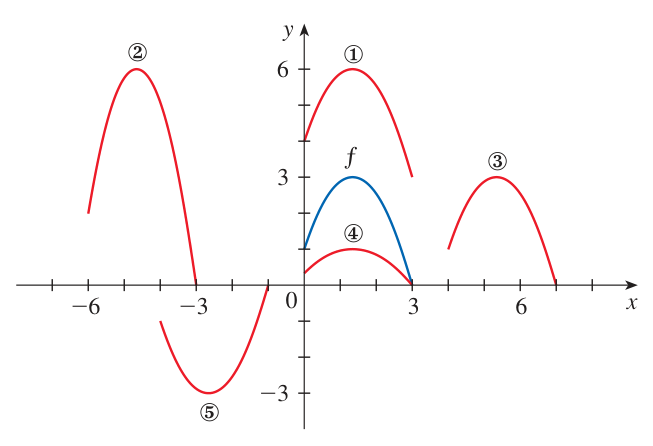
\includegraphics[width=0.88\linewidth]{images/p0077_fig1.png}
        \end{center}
    \end{enumerate}
\end{minipage}